% Applied Software Development Lab -- Lab Handout 1: Blinking LED
% Copyright (c) Michael Lehn. Licensed under CC BY-SA 4.0.
%
% Region coordinates (bp from the top of the page) follow the page layout of
% the original German handout "Laborblatt 1".
\documentclass{aslab}
\sethandout{1}{Blinking LED}
\graphicspath{{../figures/handout01/}{../figures/shared/}}

\begin{document}
%% ===================================================================== 1 ==
\maketitleblock

\begin{region}{136.0}
\heading{Learning objectives}
\end{region}

\begin{region}[pitch=13.3]{161.0}
\begin{dashlist}
\item \textbf{Working in a Unix terminal:} using basic commands such as
  \code{cat}, \code{ls}, \code{cd}, \code{pwd}, \code{mkdir}; understanding
  how the Unix file system is organized hierarchically and how to move
  around in it; creating and editing simple text files with an editor such
  as \code{nano}.
\item \textbf{Programming the microcontroller directly:} writing a simple
  program that makes an LED on a specific pin (e.g., pin~2) blink -- at
  first directly in machine code, to get a feeling for how the
  microcontroller ``understands'' programs.
\item \textbf{Measuring with the oscilloscope:} understanding why the LED no
  longer visibly blinks when the program is very fast, and how an
  oscilloscope can be used to check the actual behavior of the program.
\item \textbf{Understanding the toolchain for microcontroller programming:}
  seeing which tools are used to transfer a program to the microcontroller
  -- e.g., how \code{avr-as}, \code{avr-ld}, and \code{avr-objcopy} turn
  assembly code into machine code, and how \code{avrdude} is used to flash
  it to the microcontroller (e.g., an Adafruit Metro with an ATmega328P).
  The goal is to understand what happens ``behind the scenes'' when you
  later press a button in the Arduino IDE.
\end{dashlist}
\end{region}

\begin{region}[pitch=13.2]{391.3}
\heading{How to use this lab handout}
This lab handout is primarily a practical guide for carrying out individual
tests and experiments. It shows step by step what to do and, where useful,
contains brief notes on the meaning of individual commands or steps. The
technical background is deliberately only touched upon.
\end{region}

\begin{region}[pitch=13.3]{470.5}
A more detailed explanation of the theoretical and technical background can
be found in the separately provided \textbf{project companion}. The two
documents can be used independently of each other: for example, you can
first work through the lab handout to get a feeling for the procedures and
read up on the background afterwards -- or the other way round. Switching
back and forth between the two approaches works as well. Everyone can choose
their own way in -- depending on learning style and interest.
\end{region}

\begin{region}{589.7}
\heading{Step 1: Our first program for the ATmega328P}
\end{region}

\begin{region}{615.0}
In this step, first create a file \code{led_pin2.hex} with the following
content:
\end{region}

\begin{region}[pitch=24]{649.1}
\fontsize{21bp}{24bp}\ttfamily
:08000000529A5A9A5A98FDCF5A\par
:00000001FF
\end{region}

\begin{region}[pitch=13]{699.0}
This file contains machine code for the ATmega328P. A more detailed
explanation can be found in the \textbf{project companion}; a brief
explanation follows further below in this handout.
\end{region}

\begin{region}[pitch=12.1]{736.3}
The program \code{avrdude} can write this machine code into the program
memory of the microcontroller (this is also called ``flashing'').
\end{region}

\nextpage
%% ===================================================================== 2 ==
\begin{region}[width=368]{69.4}
\subheading{Two terminals -- why?}
For this part of the work, it is a good idea to use two terminal windows.
In the lab we use Windows PCs, but for our work we use Linux via WSL
(Windows Subsystem for Linux).
\blank
In the taskbar at the bottom of the screen you will find the icon for
opening a new Linux terminal and the overview of all terminals that are
already open.
\blank[2\baselineskip]
The best way is to open two terminals side by side -- for example like
this:
\end{region}

\placeat{436.9}{69.9}{%
\begin{tikzpicture}[x=1bp,y=-1bp,font=\fontsize{8.5bp}{9.5bp}\selectfont]
  \useasboundingbox (0,0) rectangle (110.9,76.2);
  \node[inner sep=0,anchor=north west] at (34.1,55.3)
    {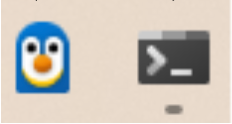
\includegraphics[width=33.2bp]{taskbar-icons.png}};
  \node[align=center,anchor=south] (new) at (16,40) {New\\terminal};
  \node[align=center,anchor=south] (all) at (84,38) {Overview of all\\open terminals};
  \draw[-{Stealth[length=3pt]},line width=0.6bp] (30.1,36.5) -- (38.7,54.5);
  \draw[-{Stealth[length=3pt]},line width=0.6bp] (70.2,36.5) -- (60.2,54.5);
\end{tikzpicture}}

\placegraphic{56.7}{192.2}{353.3}{two-terminals.png}

\placeat{427.1}{196.1}{%
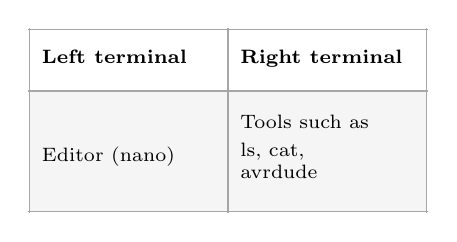
\begin{tikzpicture}[x=1bp,y=-1bp,font=\scriptsize]
  \fill[gray!8] (0.5,22) rectangle (143.3,65.4);
  \draw[gray!70!white,line width=0.5bp]
    (0,0) -- (143.8,0) (0,22) -- (143.8,22) (0,65.4) -- (143.8,65.4)
    (0.5,-0.5) -- (0.5,66) (71.9,-0.5) -- (71.9,66) (143.4,-0.5) -- (143.4,66);
  \node[anchor=base west,inner sep=0] at (4.7,12.2) {\bfseries Left terminal};
  \node[anchor=base west,inner sep=0] at (76.1,12.2) {\bfseries Right terminal};
  \node[anchor=base west,inner sep=0] at (4.7,47.3) {Editor (nano)};
  \node[anchor=north west,inner sep=0,align=left,text width=64bp]
    at (76.1,30.5) {\baselineskip=10bp Tools such as\\
      \codearg{ls}, \codearg{cat},\\\codearg{avrdude}};
\end{tikzpicture}}

\begin{region}{378.1}
The advantage: a stress-free workflow. You edit your file on the left and
test it or enter commands on the right. If, for example, an error occurs,
tools often report a line number -- and you have it right in front of you
when you make the correction on the left.
\end{region}

\begin{region}{427.1}
\subheading{Tasks:}
\end{region}

\begin{region}{452.1}
\begin{tasks}
\item \textbf{Create the file and enter its content}
  \begin{steps}
  \item In the left terminal, enter the following command:
    \blank
    \tcode{nano led_pin2.hex}
    \blank
    This starts the text editor \code{nano} with a (still empty) file
    named \code{led_pin2.hex}.
  \item Now enter the code shown above (two lines).\\
    Make sure to copy it exactly -- including the colons. The letters A--F
    may be entered in lowercase or uppercase here, but keep in mind that in
    many programming languages the case of letters does make a difference.
    By the way, a not uncommon mistake is typing \code{O} (``oh'') instead of
    \code{0} (``zero'')!
  \item Save the file with the key combination \key{Control} + \key{S}.
  \end{steps}
\end{tasks}
\end{region}

\begin{region}{610.3}
\begin{tasks}[start=2]
\item \textbf{First steps with Unix commands}\\
  In the right terminal you can now check the file:
  \begin{steps}
  \item Enter:
    \blank
    \tcode{ls}
    \blank
    This lists all files in the current directory. The file
    \code{led_pin2.hex} should now appear.
  \item Enter:
    \blank
    \tcode{cat led_pin2.hex}
    \blank
    This prints the content of the file in the terminal. Compare it with
    what you entered in nano on the left.
  \end{steps}
\end{tasks}
\end{region}

\nextpage
%% ===================================================================== 3 ==
\begin{region}{69.4}
\heading{Step 2: Connecting the microcontroller and detecting the device}
\end{region}

\begin{region}{93.5}
Before we connect the microcontroller, let us briefly look at how you can
tell under Linux whether a device (e.g., a USB-to-serial converter) has been
recognized by the system.
\end{region}

\begin{region}{130.4}
\subheading{Terminal tip:}
If you want to enter a command again in the terminal, you can simply press
the up-arrow key. This is especially handy when you run a command
repeatedly or want to modify it slightly.
\end{region}

\begin{region}{191.4}
\subheading{Tasks:}
\end{region}

\begin{region}{216.4}
\begin{tasks}
\item \textbf{Do not connect the microcontroller yet}\\
  Enter the following command in the terminal:
  \blank
  \tcode{ls /dev/*}
  \blank
  This command lists all device files located in the directory
  \code{/dev/}. Under Linux, almost everything is treated as a ``device
  file'' -- including USB devices. A USB-to-serial converter like the one on
  our microcontroller board would show up here, e.g., as
  \code{/dev/ttyUSB0}.
  \blank
  Since no microcontroller is connected yet, the output should of course
  \textbf{not} contain an entry like \code{/dev/ttyUSB0}.
\end{tasks}
\end{region}

\begin{region}{377.4}
\begin{tasks}[start=2]
\item \textbf{Connect the microcontroller}\\
  Now connect the microcontroller to the computer with the USB cable. On a
  real (native) Linux system, running
  \blank
  \tcode{ls /dev/*}
  \blank
  again would now show an additional entry such as \code{/dev/ttyUSB0} --
  that would be your device.
  \blank
  Since we are working in WSL under Windows, however, Linux runs as a
  ``guest'' here, and the USB port has to be passed through. For this
  purpose, we have prepared a helper script called \code{usb_check}.
\end{tasks}
\end{region}

\begin{region}{524.3}
\begin{tasks}[start=3]
\item \textbf{Run \codearg{usb\_check}}\\
  Enter:
  \blank
  \tcode{usb_check}
  \blank
  The script gives WSL access to the USB port. Afterwards, check again
  with:
  \blank
  \tcode{ls /dev/*}
  \blank
  whether \code{/dev/ttyUSB0} now appears. If so: everything is ready for
  flashing!
\end{tasks}
\end{region}

\begin{region}{682.2}
\subheading{What to do if there are problems?}
If \code{usb_check} reports an error or asks for the administrator password:
don't panic. Such things can happen -- especially when workarounds were
still being tinkered with shortly before the start of the semester
\emoji{1F604}\ Sit back for a moment and stay relaxed -- we will help you
shortly.
\end{region}

\nextpage
%% ===================================================================== 4 ==
\begin{region}{69.4}
\heading{Step 3: Flashing the microcontroller}
\end{region}

\begin{region}{93.5}
Now it is getting serious: we transfer our program to the microcontroller
-- that is, into its flash memory, where it is executed automatically after
power-up.\\
To do this, enter the following command in the right terminal:
\end{region}

\begin{region}{141.5}
\fontsize{10bp}{12bp}\ttfamily
avrdude -c arduino -P /dev/ttyUSB0 -p atmega328p -U flash:w:led\_pin2.hex:i
\end{region}

\begin{region}{165.5}
If everything works, the output of \code{avrdude} looks roughly like this:
\end{region}

\placegraphic{56.7}{180.2}{361.1}{avrdude-output.png}

\begin{region}{446.4}
Now we make a small case distinction -- just like when programming with
\code{if} and \code{else}:
\end{region}

\begin{region}{482.8}
\begin{bullets}
\item If the output contains something like:
  \blank
  \tcode{8 bytes of flash written}\\
  \tcode{8 bytes of flash verified}
  \blank
  then flashing was successful. Continue with the next step!
\end{bullets}
\end{region}

\begin{region}{567.0}
\begin{bullets}
\item If, on the other hand, \code{avrdude} reports an error -- or
  ``verifying failed'' appears -- then:
  \blank
  \textbf{Back to Step 1!} Most likely a typo crept in while you were
  entering the hex file. Go back to \code{nano}, check everything, save
  again, and then try once more.
\end{bullets}
\end{region}

\begin{region}{641.4}
\subheading{Errors are part of the workflow}
Errors during flashing (or during programming in general) are completely
normal. What matters is that you understand them \textbf{as part of the
workflow}:
\end{region}

\begin{region}[pitch=12.6]{689.8}
\begin{dashlist}
\item You recognize that an error has occurred (e.g., from unusual
  \code{avrdude} output),
\item you learn not to overlook such messages, but eventually to notice
  them even subconsciously -- the way you notice a red traffic light
  without consciously looking at it,
\item and you know which step you have to go back to in order to fix it.
\end{dashlist}
\end{region}

\begin{region}{762.4}
This is exactly what working professionally means: errors are not a step
backwards -- they are the way to the solution.
\end{region}

\nextpage
%% ===================================================================== 5 ==
\placefigure[198.8]{363.1}{59.2}{175.5}{flowchart-led.tex}

\begin{region}[width=294]{69.4}
\heading{Step 4: Measuring what the program does}
\blank
Congratulations -- you have made it to Step~4!\\
The machine program has already been transferred successfully to the
microcontroller and is running now. So it is about time to find out what we
have actually done there.
\blank
You can find the details in the project companion -- but, as everyone
knows, people like to read a manual only afterwards. So here is the most
important information in brief. Our program consists of exactly four
machine instructions:
\end{region}

\begin{region}{224.9}
\begin{dashlist}
\item set pin~2 as an output
\item set pin~2 HIGH
\item set pin~2 LOW
\item and a jump instruction
\end{dashlist}
\end{region}

\figcaption{396.6}{279.5}{Fig. 1: Flowchart}

\begin{region}{309.5}
These instructions are executed one after the other, as shown in
Figure~1. Each of these instructions takes two CPU clock cycles. At a clock
frequency of 16\,MHz, one clock cycle lasts exactly 62.5\,ns. This means:
pin~2 should be HIGH for 125\,ns, then LOW for 250\,ns -- and then the
sequence starts all over again. Figure~2 sketches this sequence.
\end{region}

\placefigure{56.7}{360.2}{340.9}{signal-pin2.tex}

\figcaption{160.7}{474.2}{Fig. 2: Signal at pin~2.}

\begin{region}{505.3}
\textbf{But anyone can claim that. We, however, measure it -- with the
oscilloscope!}
\end{region}

\placegraphic{46.3}{520.6}{218.5}{oscilloscope-setup.jpg}
\placegraphic{274.6}{520.6}{264.0}{oscilloscope-screen.png}

\begin{region}[pitch=12.3]{708.5}
\begin{tabular}[t]{@{}p{12bp}@{\hspace{6bp}}p{192bp}@{}p{265.9bp}@{}}
\textbf{1.} & Connect the probe: &
  Channel 1 (yellow) to pin~2 of the microcontroller, ground lead (cable
  with alligator clip) to \code{GND}.\\
\textbf{2.} & Set the trigger: &
  Mode: \code{Edge}, Source: \code{Chan 1}, Level approx.\ 2.5\,V\\
\textbf{3.} & Adjust the time base: &
  \code{Time/Div}: approx.\ 100\,ns\\
\textbf{4.} & Enable automatic measurement: &
  Press the \code{Meas} key and select one after the other:\newline
  \code{+Width} (measures the HIGH duration),\newline
  \code{-Width} (measures the LOW duration)
\end{tabular}
\end{region}

\nextpage
%% ===================================================================== 6 ==
\begin{region}{81.4}
\heading{Step 5: A small hack in the machine code}
\blank
The project companion explains the so-called Intel HEX format in detail.
Here is the short version. The file \tcode{led_pin2.hex} contains more than
just the actual program. In addition to the machine program, it contains,
for example:
\end{region}

\begin{region}{140.9}
\begin{dashlist}
\item how many bytes are to be transferred
\item the address to which they are to be written
\item a checksum for error detection
\end{dashlist}
\end{region}

\begin{region}{189.5}
The first line, for example, has the following structure:
\end{region}

\placefigure{56.7}{204.2}{481.9}{hexrecord-led.tex}

\begin{region}{269.9}
The machine program itself consists only of the bytes highlighted in green:
\end{region}

\begin{region}{294.1}
{\setlength\fboxsep{0pt}\colorbox{hlgreen!45}{\vrule width0pt height 9.6bp
  depth 2.4bp\ttfamily 529a5a9a5a98fdcf}}
\end{region}

\begin{region}{317.9}
By the way, the second line of the file (\tcode{:00000001FF}) simply means:
no more data follows.
\end{region}

\begin{region}{342.8}
\textbf{Now here comes the clever part:} The checksum in the Intel HEX
format detects many kinds of transmission errors -- but not all of them. If
two consecutive instructions are swapped, the behavior of the program
changes -- but the checksum stays the same.
\end{region}

\begin{region}{391.8}
\subheading{Task:}
In \tcode{led_pin2.hex}, swap the instructions for ``set pin~2 HIGH'' and
``set pin~2 LOW''. If everything works, you should see on the oscilloscope:
250\,ns HIGH and 125\,ns LOW.
\end{region}

\begin{region}{440.8}
\textbf{Difference from Step 4:} There, we measured in order to understand
what happens. Now we make a prediction and then check whether it is
correct.
\end{region}

\placefigure[285.4]{375.8}{476.0}{176.0}{flowchart-led-symmetric.tex}

\begin{region}[width=294,pitch=12.95]{489.8}
\heading{Step 6: A hack for a symmetric signal}
\blank
The project companion explains how to modify the program so that pin~2 is
\textbf{HIGH for 250\,ns} and then \textbf{LOW for 250\,ns}.
\blank
The signal then consists of phases of \textbf{equal length} -- it is
therefore \textbf{symmetric} and has a clean frequency.
\end{region}

\begin{region}[width=294]{601.9}
To achieve this, we simply insert two additional instructions, so-called
\textbf{NOPs}:
\begin{dashlist}
\item NOP stands for ``No Operation'' -- that is, ``do nothing''.
\item The instruction takes one CPU clock cycle but does not change
  the state of the pin:
  \begin{dashlist}
  \item If pin~2 is HIGH, it stays HIGH.
  \item If it is LOW, it stays LOW.
  \end{dashlist}
\end{dashlist}
\end{region}

\begin{region}[width=294]{698.9}
In our case, we insert the two NOPs directly after the ``set pin HIGH''
instruction. This extends the HIGH phase by
\blank
\hspace*{36bp}125\,ns + 125\,ns = 250\,ns.
\blank
Figure~3 shows exactly what this looks like.
\end{region}

\figcaption{396.6}{783.1}{Fig. 3: Symmetric signal}

\nextpage
%% ===================================================================== 7 ==
\begin{region}{80.5}
The new program now consists of the following bytes:
\blank
\tcode{529A5A9A000000005A98FBCF}
\end{region}

\begin{region}{128.5}
So, in summary:\\
In \code{led_pin2.hex}, only the first line needs to be changed.
\blank
The only tricky part: what is the new checksum?
\end{region}

\placefigure{56.7}{179.5}{272.1}{hexrecord-new.tex}

\begin{region}{232.4}
Of course, you could look up in the project companion exactly how it is
calculated. But here, the essentials are enough:
\end{region}

\begin{region}[x=70.9]{268.4}
First, all bytes except the checksum are added up -- always calculating
with two hex digits, i.e., with 8-bit overflow: higher digits are simply
cut off. The checksum is then exactly the number that would still have to
be added so that the result is 0 again.
\end{region}

\begin{region}[pitch=13]{329.4}
The crucial point for us: we only need to look at \textbf{where something
has changed} and \textbf{by how much the sum has changed}.
\end{region}

\placefigure{56.7}{345.1}{271.2}{hexrecord-changes.tex}

\begin{region}{436.3}
And these are exactly three things:
\end{region}

\begin{region}[pitch=12.3]{460.3}
\begin{tasks}
\item The number of bytes has increased by 4.
\item The two new NOP instructions (\code{00 00 00 00}) contribute 0 to the
  sum.
\item The jump instruction has changed: \code{FD CF} becomes \code{FB CF},
  i.e., the first byte is smaller by 2.
\end{tasks}
\end{region}

\begin{region}[pitch=13.3]{521.0}
So the sum has become smaller by 2\\
$\rightarrow$ the checksum must therefore become larger by 2 to compensate.\\
$\rightarrow$ The old checksum was 5A, so the new one should be 58.
\end{region}

\begin{region}{584.6}
\subheading{Task:}
\blank
Modify \code{led_pin2.hex} by
\end{region}

\begin{region}{620.4}
\begin{dashlist}
\item inserting the new machine instructions,
\item increasing the data length accordingly,
\item and changing the checksum from 5A to 58.
\end{dashlist}
\end{region}

\begin{region}{668.9}
If we have made neither a reasoning error nor a calculation error,
\code{avrdude} will accept the checksum without complaint, and the
oscilloscope will show a symmetric signal.
\end{region}

\nextpage
%% ===================================================================== 8 ==
\begin{region}{69.4}
\heading{Intermezzo: A look at the end}
\blank
In Step~7 we clone a finished game and play it together. Not because we
want to analyze the code -- but to get an impression of where this course is
heading. What you are about to play is an example of what is possible at
the end:
\end{region}

\begin{region}{142.4}
\textbf{A self-written game in Python that can be controlled with a
microcontroller.}
\end{region}

\begin{region}{166.5}
What exactly you program is, of course, up to you. For classics such as
Pong or Breakout (the game in which you bounce a ball off a paddle at the
bottom and hit blocks at the top), there will be step-by-step instructions
-- but also plenty of room for your own ideas.
\end{region}

\begin{region}{214.5}
Over the course of the semester, we move from hardware-oriented programming
(machine code, assembly language, ports, timing~\dots) all the way to
platform-independent software development in Python. The point is not to
memorize solutions, but to understand which problem is being solved in each
case -- and why a particular approach makes sense. Once you know the
problem, you also understand the purpose of the solution -- whether it is
about assembly language, C, or object-oriented programming. And you can
better judge when and how to use such tools sensibly.
\end{region}

\begin{region}{311.4}
\heading{Step 7: Playing TRON Lightcycle}
\blank
To round off the first session, we play a game!
\end{region}

\begin{region}[pitch=13]{360.4}
At first glance, the game may remind you of Snake -- but it has different
roots: \textbf{TRON} was a science fiction film from 1982 and the first
feature film to make extensive use of \textbf{computer-generated imagery
(CGI)}. Its lightcycle races have inspired many game ideas -- including
this one.
\end{region}

\begin{region}{423.4}
\subheading{Tasks}
\end{region}

\begin{region}{447.5}
\begin{tasks}
\item The game is available on GitHub at:
  \link{https://github.com/michael-lehn/tron.git}
  \blank
  To clone it, enter the following in the terminal:
  \blank
  \tcode{git clone https://github.com/michael-lehn/tron.git}
\end{tasks}
\end{region}

\begin{region}{520.8}
\begin{tasks}[start=2]
\item \textbf{Who does what?}\\
  The game can be played by four people -- which fits perfectly, because
  the lab has four computers per row. One of you starts the server, the
  others connect to it with the client.
\end{tasks}
\end{region}

\begin{region}[x=74.7,right=0]{581.8}
\begin{list}{}{\leftmargin=18bp\labelwidth=18bp\labelsep=0pt\itemsep=0pt
  \parsep=0pt\topsep=0pt}
\item[\bfseries(A)\hfill] \textbf{Starting the server:} Open a terminal,
  change into the directory, and start the server:
  \blank
  \tcode{cd tron}\\
  \tcode{python new-tron-server.py 1000 1000 4}
  \blank
  This starts a game on a 1000\,\texttimes\,1000 grid for four players.
  Whoever starts the server should also look up their own IP address and
  tell it to the others:
  \blank
  \tcode{curl -4 ifconfig.me}
\end{list}
\end{region}

\begin{region}[x=74.7,right=0]{703.1}
\begin{list}{}{\leftmargin=18bp\labelwidth=18bp\labelsep=0pt\itemsep=0pt
  \parsep=0pt\topsep=0pt}
\item[\bfseries(B)\hfill] \textbf{Starting the client:} The clients are
  started on each computer as follows:
  \blank
  \tcode{cd tron}\\
  \tcode{python tron-2d.py}\hspace{3em}(or \tcode{python tron-3d.py})
  \blank
  On the start screen, you can then enter your name and the IP address of
  the server.
\end{list}
\end{region}

\end{document}
